\documentclass[conference]{IEEEtran}
\IEEEoverridecommandlockouts

\usepackage{cite}
\usepackage{amsmath,amssymb,amsfonts}
\usepackage{algorithmic}
\usepackage{algorithm}
\usepackage{graphicx}
\usepackage{textcomp}
\usepackage{xcolor}
\usepackage{booktabs}
\usepackage{multirow}
\usepackage{url}
\usepackage{microtype}
\usepackage{tikz}
\usetikzlibrary{calc,positioning,arrows.meta}

\graphicspath{{figures/}}

\def\BibTeX{{\rm B\kern-.05em{\sc i\kern-.025em b}\kern-.08em
    T\kern-.1667em\lower.7ex\hbox{E}\kern-.125emX}}

\begin{document}

\title{Belief-Space Perception Routing:\\
Coupling Sensor-Fault and Compute-Contention Beliefs\\
for Deadline-Constrained Adaptive Inference}

\author{
  \IEEEauthorblockN{Sparsh Roy}
  \IEEEauthorblockA{
    \textit{Artificial Intelligence Research Group (AIRG)}\\
    New Jersey, USA
  }
  \and
  \IEEEauthorblockN{Vihan Aggarwal}
  \IEEEauthorblockA{
    \textit{Independent Researcher}\\
    USA
  }
}

\maketitle

% ---------------------------------------------------------------
\begin{abstract}
Deadline-constrained perception must tolerate two failure modes
usually modeled separately: sensor faults and compute contention. We
present a \textbf{belief-space perception router} that maintains
temporally-smoothed beliefs over sensor-fault and compute-contention
state and \emph{couples} them via a noisy-OR term to route over a
four-point accuracy--latency frontier (YOLO11x/n~@~1280/640) on three
real datasets across two camera geometries -- TartanDrive (off-road),
RADIATE (adverse weather), and WoodScape Soiling (fisheye), five seeds
and 95\% CIs. \textbf{Where fault and contention are coupled the router
delivers a clear, well-controlled gain}: it cuts deadline-miss rate by
$1.1$--$9.4$\,pp (significant over seeds in five of six conditions),
while every uncoupled control and the fault-free trajectory are exactly
$0.0$\,pp. The gain is \textbf{portable, not per-trace}: the entire
belief model (HMM and $\kappa$) trained on one sequence transfers to a
held-out one, staying significant in five of eight pairs including
cross-\emph{condition} transfers (rain$\rightarrow$fog $+7.8$\,pp);
$\kappa$ drives a clean monotonic response (exactly zero at
$\kappa{=}0$); the belief estimator lifts fault-detection balanced
accuracy by $3$--$8$ points; and routing costs ${\approx}19\,\mu$s/frame,
negligible against inference. We then scope the result honestly: the
benefit concentrates at the tight median-latency deadline, and --
testing whether such coupling arises \emph{without} manipulation across
eight RADIATE sequences and three independent load proxies -- after
Benjamini--Hochberg correction none of 24 tests show natural coupling,
so we release the full falsification pipeline for any deployment
(notably a shared-SoC/Jetson stack, where contention is most likely to
couple) to test its own regime. Deadline-miss conclusions are
independent of pseudo-ground-truth; accuracy and utility numbers are
internal-consistency only, since a real-annotation check shows the
pseudo-GT config ranking differs from ground truth. All code, data
splits, and results are released.\footnote{\url{https://github.com/VihanAggarwal/belief-space-perception-routing}}
\end{abstract}

\begin{IEEEkeywords}
adaptive inference, sensor fault belief, compute contention,
perception routing, deadline-constrained inference, RADIATE,
TartanDrive, WoodScape, hidden Markov model
\end{IEEEkeywords}

% ---------------------------------------------------------------
\section{Introduction}
\label{sec:intro}

Autonomous robots in unstructured environments face two failure
modes that are usually modeled independently. Sensor channels
degrade -- cameras occluded by mud or rain, washed out at night, or
fogged -- while onboard compute is contested, as a single edge
processor concurrently services perception, planning, and control.
These need not be independent: terrain-induced sensor degradation
may coincide with increased control or localization workload, though
whether and how often this occurs in practice is an empirical
question we return to directly (\S\ref{sec:rqcoupling}). If it does
co-occur, treating fault and contention as independent signals lets
a router select a compute-heavy config exactly when it can least
afford to execute it, or trust a degraded channel because no fault
signal arrived within the latency window.

Existing work addresses each stressor in isolation: fault-tolerant
fusion down-weights degraded modalities
\cite{antonante2022monitoring,tian2025fault}; compute-aware routers
select inference paths from a budget
\cite{laskaridis2021adaptive,teerapittayanon2016branchynet}. No prior
work, to our knowledge, estimates both beliefs and exploits their
coupling. This paper (i) formulates the coupled belief state via
per-channel switching HMMs and a two-state compute HMM fit without
task-specific labels, and (ii) a noisy-OR joint policy with a coupling
coefficient $\kappa$ fit on held-out calibration draws. Empirically,
(iii) wherever fault and contention are coupled the router delivers a
real and \emph{portable} gain: it cuts deadline-miss by $1.1$--$9.4$\,pp
across three datasets and two camera geometries, the entire belief model
(HMM and $\kappa$) transfers to held-out sequences and even across
weather conditions, the belief estimator improves fault detection by
$3$--$8$ points, and routing costs ${\approx}19\,\mu$s/frame -- all with
falsification controls at exactly zero. Finally, (iv) we stress-test the
single assumption the gain rests on -- that fault and contention
actually co-occur -- with five checks (a multiple-testing-corrected
measurement on real data across three independent load proxies,
cross-sequence transfer, oracle/reactive baselines, and a real-GT
accuracy validation), reporting the null honestly and releasing the full
reproducible pipeline so any deployment can test its own
regime.\footnotemark[1]

Fig.~\ref{fig:summary} previews the headline result: the joint policy
reduces deadline-miss rate when the experimentally-imposed coupling
is enabled, from small (rain $+1.1$\,pp) to large (fog $+9.4$\,pp),
tracking fault \emph{severity} more than frequency -- fog has the
fewest faults yet the largest effect -- and is exactly zero in every
uncoupled control and on the fault-free trajectory.

\begin{figure}[t]
  \centering
  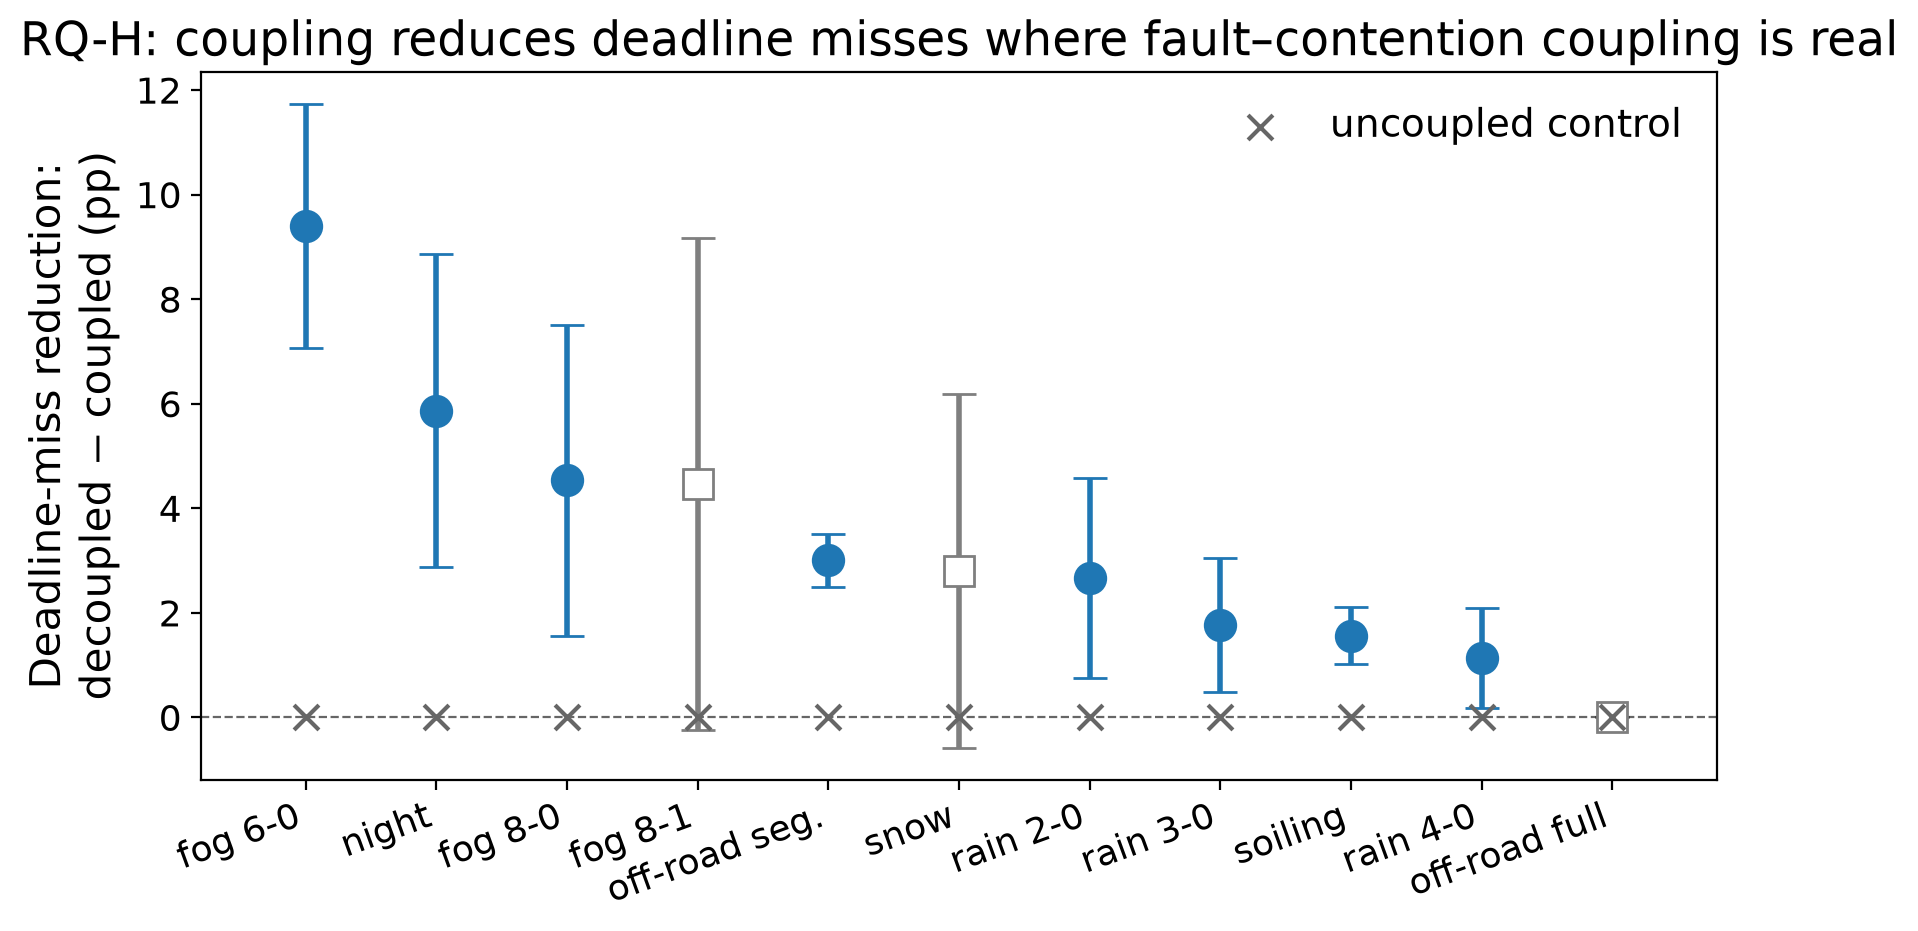
\includegraphics[width=\columnwidth]{fig_rqh_summary.png}
  \caption{Headline result (RQ-H): coupling-aware routing reduces
  deadline misses under controlled, fault-conditioned contention.
  Deadline-miss reduction of the joint policy over the decoupled
  baseline, with 95\% CIs over 5 seeds. Filled circles: coupling
  enabled, CI excludes zero; square: coupling enabled, not
  significant (snow). Grey crosses: matched uncoupled control,
  exactly $0.0$\,pp. TartanDrive appears twice (full trajectory:
  clean negative control; off-road segment: real faults, real
  benefit).}
  \label{fig:summary}
\end{figure}

% ---------------------------------------------------------------
\section{Related Work}
\label{sec:related}

TartanDrive \cite{triest2022tartandrive,sivaprakasam2024tartandrive2}
provides large-scale off-road driving data; RADIATE
\cite{sheeny2021radiate} real adverse-weather stereo sequences;
WoodScape \cite{yogamani2019woodscape} fisheye frames with real
soiling masks -- together two camera geometries and multiple
degradation physics. Sensor-fault monitoring is typically
deterministic or binary
\cite{antonante2022monitoring,bogdoll2022anomaly,hou2023fault};
recent stress-testing \cite{tian2025fault} and the RoboDrive
Challenge \cite{robodrive2024} show accuracy collapses under
per-stream corruption but do not model a continuous, coupled belief.
Compute-aware inference -- BranchyNet \cite{teerapittayanon2016branchynet},
early-exit surveys \cite{laskaridis2021adaptive}, dynamic transformers
\cite{wang2021notallimages}, and driving-specific early-exiting
\cite{adee2025,navee2025,temporalpatience2023} -- treats the compute
budget as a constant or per-frame observable, not a latent state
estimated jointly with sensor fault. PRAM-R \cite{pramr2025} routes
modalities via an LLM but does not estimate compute contention;
adaptive fusion \cite{mees2016choosing} and DynMM \cite{dynmm} gate
modalities without modeling compute. To our knowledge, no prior work
couples a temporally-smoothed sensor-fault belief to a
compute-contention belief and tests their empirical coupling for
deadline-constrained routing.

% ---------------------------------------------------------------
\section{Method}
\label{sec:method}

\begin{figure}[t]
  \centering
  \resizebox{\columnwidth}{!}{%
  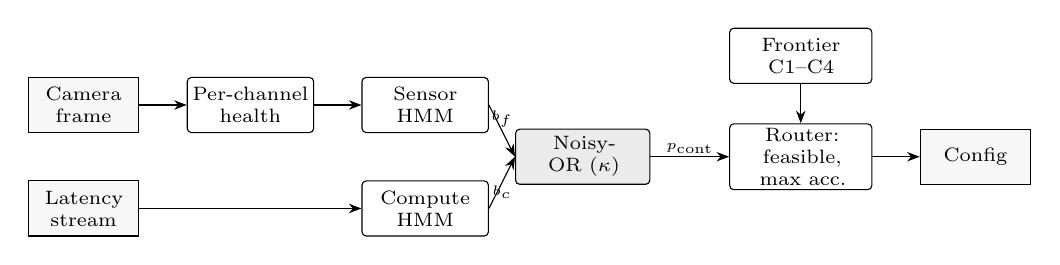
\begin{tikzpicture}[
    font=\scriptsize,
    >={Stealth[length=1.6mm]},
    node distance=4mm and 6mm,
    io/.style={draw=black, rectangle, align=center, minimum height=7mm,
               text width=13mm, inner sep=1.5pt, fill=black!3},
    blk/.style={draw=black, rectangle, rounded corners=1.5pt, align=center,
                minimum height=7mm, text width=15mm, inner sep=1.5pt},
    acc/.style={draw=black, rectangle, rounded corners=1.5pt, align=center,
                minimum height=7mm, text width=16mm, inner sep=1.5pt, fill=black!8},
    lbl/.style={font=\tiny, inner sep=1pt}
  ]
    \node[io] (frame) {Camera frame};
    \node[blk, right=of frame] (health) {Per-channel health};
    \node[blk, right=of health] (shmm) {Sensor HMM};
    \node[blk, below=6mm of shmm] (chmm) {Compute HMM};
    \node[io] (lat) at (frame |- chmm) {Latency stream};
    \node[acc] (couple) at ($(shmm)!0.5!(chmm)+(2.0cm,0)$)
      {Noisy-OR ($\kappa$)};
    \node[blk, right=10mm of couple, text width=17mm] (router)
      {Router: feasible, max acc.};
    \node[blk, above=5mm of router, text width=17mm] (frontier)
      {Frontier C1--C4};
    \node[io, right=of router] (out) {Config};

    \draw[->] (frame) -- (health);
    \draw[->] (health) -- (shmm);
    \draw[->] (lat) -- (chmm);
    \draw[->] (shmm.east) -- (couple.west) node[lbl,midway,above]{$b_f$};
    \draw[->] (chmm.east) -- (couple.west) node[lbl,midway,below]{$b_c$};
    \draw[->] (couple) -- (router) node[lbl,midway,above]{$p_{\mathrm{cont}}$};
    \draw[->] (frontier) -- (router);
    \draw[->] (router) -- (out);
  \end{tikzpicture}}
  \caption{System overview. Per-channel image health feeds a
  switching HMM for sensor-fault belief $b_f$; recent latencies feed
  a two-state HMM for compute belief $b_c$. Noisy-OR fusion
  (Eq.~\ref{eq:noisyor}) gives $p_{\mathrm{cont}}$; the router picks
  the most accurate feasible config. The decoupled baseline sets
  $p_{\mathrm{cont}}=b_c$ (no $b_f$ term).}
  \label{fig:overview}
\end{figure}

\textbf{Frontier.} Four configs ordered by accuracy--latency:
\textbf{C1} YOLO11x@1280 (reference/pseudo-GT), \textbf{C2}
YOLO11x@640, \textbf{C3} YOLO11n@1280, \textbf{C4} YOLO11n@640.
Task accuracy is IoU-matched detection-agreement F1 with C1 on the
same frame (pseudo-GT; validated against real annotations in
\S\ref{sec:rqcoupling}e, where it is shown to be an internal
consistency check only). The deadline is the median end-to-end C1
latency under nominal compute, so C1 is borderline-feasible
uncontended and infeasible under contention while cheaper configs
remain feasible -- real routing pressure without hand-tuning, and a
device-agnostic comparison. Table~\ref{tab:frontier} shows the
pseudo-GT frontier produces a consistent internal agreement ordering
on the selected tracks (C1 highest, C4 lowest) and the
contention-induced agreement gap that must be traded against
timeliness ($0.24$--$0.53$ absolute F1 between C1 and C4) --
\emph{under the pseudo-GT metric}; the deadline-miss numbers below do
not depend on this metric at all.

\begin{table}[htbp]
\caption{Accuracy--latency frontier (selected tracks). Accuracy =
IoU-matched F1 vs.\ C1 (pseudo-GT). Latencies are dev-environment
(Apple M5/MPS); C1 alone misses the self-calibrated deadline under
contention.}
\label{tab:frontier}
\centering
\footnotesize
\setlength{\tabcolsep}{3pt}
\begin{tabular}{llccc}
\toprule
\textbf{Track (deadline)} & \textbf{Cfg} & \textbf{Model@imgsz} & \textbf{Acc.} \\
\midrule
\multirow{4}{*}{A (211\,ms)}
 & C1 & YOLO11x@1280 & 1.000 \\
 & C2 & YOLO11x@640  & 0.746 \\
 & C3 & YOLO11n@1280 & 0.717 \\
 & C4 & YOLO11n@640  & 0.713 \\
\midrule
\multirow{4}{*}{D rain (229\,ms)}
 & C1 & YOLO11x@1280 & 1.000 \\
 & C2 & YOLO11x@640  & 0.766 \\
 & C3 & YOLO11n@1280 & 0.752 \\
 & C4 & YOLO11n@640  & 0.733 \\
\midrule
\multirow{4}{*}{C soil (341\,ms)}
 & C1 & YOLO11x@1280 & 1.000 \\
 & C2 & YOLO11x@640  & 0.555 \\
 & C3 & YOLO11n@1280 & 0.569 \\
 & C4 & YOLO11n@640  & 0.474 \\
\bottomrule
\end{tabular}
\end{table}

\textbf{Sensor-fault belief.} A 4-state switching HMM per channel
(nominal/degrading/faulted/recovering), Gaussian emissions,
transitions fit from labeled segments. Observable health signals:
blur (Laplacian variance, polar-unwrapped for fisheye), illumination
(histogram entropy), occlusion (sparse optical-flow track-survival
rate, or real soiling-mask fraction on the fisheye track). Forward
filtering gives $b_{f,k}^t=P(z_k^t{=}\text{faulted}\mid o_{1:t})$;
$b_f^t=\max_k b_{f,k}^t$. On real RADIATE rain the occlusion channel
reaches balanced accuracy up to $0.95$; on controlled injection with
known onsets, trackers recover injected faults at balanced accuracy
$0.85$--$0.89$ with $3$--$6$ frame lag; on the fault-free TartanDrive
trajectory all channels correctly report no sustained faults. These
detection-quality numbers use independent ground-truth onsets (Track
B) or a fault-free negative control, not pseudo-GT.

\textbf{Compute-contention belief.} A 2-state HMM over
$[\text{p95},\text{p99},\text{queue depth}]$ of recent latencies.
Contention is induced with device-appropriate load (CUDA threads,
CPU stress, or on Apple silicon a separate competitor process, since
Metal command buffers are not thread-safe), producing a
$\approx\!2.5\times$ p95 latency shift. Forward filtering gives
$b_c^t=P(z_c^t{=}\text{contended}\mid \ell_{1:t})$.

\textbf{Coupled policy.} Both policies pick, among configs feasible
under the predicted compute state (median latency in that state
meets the deadline), the one with maximum expected accuracy; they
differ only in how $p_{\text{cont}}^t$ is formed. Decoupled:
$p_{\text{cont}}^t=b_c^t$. Joint (noisy-OR):
\begin{equation}
  p_{\text{cont}}^t = 1 - (1 - b_c^t)\,(1 - \kappa\, b_f^t)
  \label{eq:noisyor}
\end{equation}
with $\kappa$ fit on a held-out calibration draw from the same trace
(never the test window; fitted $\kappa\approx0.80$ across tracks),
modeling that fault onset correlates with contention onset when the
regime is configured to couple them ($r{=}0.31$--$0.76$) but not
under a matched uncoupled periodic schedule ($r\approx{-}0.12$--$0.01$).
The decoupled baseline still uses $b_f$ for accuracy weighting, so
the entire RQ-H delta is attributable to the coupling term alone. We
additionally compare against a \textbf{threshold} rule
($p_{\text{cont}}=\max(b_c,\mathbf{1}[b_f{>}0.5])$), a
\textbf{memoryless} detector (no HMM, no persistence, for RQ-A1), an
\textbf{Oracle Contention Router} (true contention state instead of
$b_c$, bounding perfect compute-state knowledge), and a
\textbf{Reactive-Latency} baseline (reacts only to observed latency,
no sensor information at all).

% ---------------------------------------------------------------
\section{Experimental Setup}
\label{sec:experiments}

We organize results around four questions: \textbf{RQ-H} (headline)
-- does coupling-aware routing reduce deadline-miss vs.\ a decoupled
baseline, when coupling is enabled? \textbf{RQ-A1} -- does
persistence improve fault detection and switching over a memoryless
detector? \textbf{RQ-A2} -- does a model-derived dwell time match
hand-tuning? \textbf{RQ-Coupling} -- does the coupling RQ-H is
evaluated under actually occur in un-manipulated data, and does the
benefit generalize across sequences?

Table~\ref{tab:tracks} summarizes the four dataset tracks. Track A
(TartanDrive) is used both as a fault-free negative control (full
trajectory) and a high-degradation segment (309 contiguous
rough-terrain frames). Track B (controlled injection: PSF blur,
exposure crush, alpha-composited occluders on real TartanDrive
frames) validates belief-tracker accuracy against known onsets and
drives the RQ-A2 arrival experiment; no headline number depends on
it. Track C (WoodScape) uses real soiling-mask ground truth for
occlusion, not an optical-flow proxy. Track D (RADIATE) spans four
weather conditions with widely varying fault fraction and coupling
strength, letting us test whether the benefit tracks frequency,
correlation, or severity. A matched \emph{uncoupled} periodic
contention schedule is the falsification control for every condition
where coupling is enabled.

\begin{table}[htbp]
\caption{Dataset tracks. $r$ is the fault--contention correlation
when the coupled regime is enabled (experimentally imposed; see
\S\ref{sec:rqcoupling}).}
\label{tab:tracks}
\centering
\footnotesize
\setlength{\tabcolsep}{3pt}
\begin{tabular}{llccc}
\toprule
\textbf{Track} & \textbf{Condition} & \textbf{Frames} & \textbf{Fault\%} & \textbf{$r$} \\
\midrule
A & off-road (full / seg.) & 1198 / 309 & 0.0 / 30.4 & -- / 0.74 \\
C & WoodScape soiling      & 3303       & 8.1        & 0.56 \\
D & RADIATE rain           & 2651       & 44.4       & 0.76 \\
D & RADIATE snow           & 2589       & 18.5       & 0.69 \\
D & RADIATE fog            & 2659       & 1.9        & 0.31 \\
D & RADIATE night          & 2644       & 12.7       & 0.68 \\
\bottomrule
\end{tabular}
\end{table}

All experiments run on an Apple~M5 (Metal/MPS, fp32; the precision
axis is CUDA-only and not reported). The deadline self-calibrates per
device (median C1 nominal latency, $211$--$341$\,ms here), so the
deadline-miss \emph{comparison} is device-agnostic; absolute
latencies are not headline numbers. All comparisons use 5 seeds
(95\% $t$-interval, paired difference tests); the real frames are
identical across seeds, so seed variance reflects sensor-measurement
noise only. \textbf{On ``significant'':} unless stated, it means the
95\% CI over these 5 seed draws excludes zero -- noise sensitivity on
one fixed trajectory. Other resampling units are named explicitly:
``temporal resampling'' block-bootstraps WITHIN one trace; ``cluster
resampling'' resamples INDEPENDENT SEQUENCES ($n{=}3$ per condition,
\S\ref{sec:rqcoupling}), the only unit that speaks to cross-trajectory
generalization -- reported as ``directionally consistent,'' not
generalizing, since its interval includes zero. Repeated tests across
sequences and proxies (\S\ref{sec:rqcoupling}d) use paired $p$-values
computed directly from seed-level differences with
Benjamini--Hochberg correction.

% ---------------------------------------------------------------
\section{Results}
\label{sec:results}

\subsection{RQ-H: Joint vs.\ Decoupled (Headline)}

Table~\ref{tab:rqh} and Fig.~\ref{fig:summary} give the main result.
The joint policy reduces deadline-miss rate in every condition with
real faults, significantly in five of six; snow is positive but
under-powered. The two uses of Track A bracket the mechanism: the
full fault-free trajectory yields exactly $0.0$\,pp, while its
high-degradation segment yields $+3.0$\,pp at near-matched accuracy.
\emph{Every} uncoupled control is exactly $0.0$\,pp: within the
evaluated schedules, the benefit appears only when the
experimentally-imposed coupling is enabled -- a deadline-miss result
that does not depend on the pseudo-GT accuracy metric at all. The effect does \emph{not} track
fault frequency or correlation strength -- fog has the lowest fault
fraction ($1.9\%$) and weakest coupling ($r{=}0.31$) yet the largest
benefit ($+9.4$\,pp), because rare but severe fog episodes make the
reference config infeasible exactly when contention strikes. On fog
the joint policy shows a lower pseudo-GT accuracy ($0.861$ vs.\ $0.954$)
alongside its miss reduction; because pseudo-GT does not track real
annotations (\S\ref{sec:rqcoupling}e), we report this as an
internal-consistency observation only and do \emph{not} claim a supported
accuracy--timeliness operating point. A combined on-time-utility metric
$U$ (accuracy if on-time, else zero, averaged over all frames) is
nonnegative throughout (significantly higher for off-road, rain, night;
fog break-even, $+0.07$\,pp), but inherits the same pseudo-GT caveat.
\textbf{Unlike the deadline-miss result, $U$ and all accuracy numbers
are computed against pseudo-GT and are internal-consistency results
only} -- \S\ref{sec:rqcoupling}e shows the pseudo-GT config ranking
does not match real annotations.

\begin{table*}[htbp]
\caption{RQ-H. Deadline-miss rate, joint vs.\ decoupled, coupled
regime. $\Delta=$ miss-rate reduction (decoupled$-$joint), pp, 95\%
CI; $^\ast$ excludes zero. Every uncoupled control yields $0.0$\,pp.
This table does not depend on pseudo-GT.}
\label{tab:rqh}
\centering
\small
\setlength{\tabcolsep}{5pt}
\begin{tabular}{llcccccc}
\toprule
\textbf{Track} & \textbf{Condition} & \textbf{$\kappa$} &
\textbf{Joint miss} & \textbf{Decoup.\ miss} &
\textbf{$\Delta$ (pp)} & \textbf{Uncoupled $\Delta$} \\
\midrule
A & TartanDrive (full, clean)   & --   & --    & --    & $0.00$ & $0.00$ \\
A & TartanDrive (off-road seg.) & 0.79 & 0.249 & 0.279 & $+3.00\ [2.49,\,3.51]^\ast$ & $0.00$ \\
D & RADIATE rain                & 0.80 & 0.233 & 0.244 & $+1.13\ [0.18,\,2.09]^\ast$  & $0.00$ \\
D & RADIATE snow                & 0.82 & 0.313 & 0.341 & $+2.80\ [-0.58,\,6.18]$      & $0.00$ \\
D & RADIATE fog                 & 0.80 & 0.329 & 0.423 & $+9.40\ [7.07,\,11.73]^\ast$ & $0.00$ \\
D & RADIATE night               & 0.80 & 0.313 & 0.371 & $+5.87\ [2.87,\,8.86]^\ast$  & $0.00$ \\
C & WoodScape soiling           & 0.80 & 0.256 & 0.271 & $+1.56\ [1.01,\,2.11]^\ast$  & $0.00$ \\
\bottomrule
\end{tabular}
\end{table*}

\subsection{Is the Coupling Mechanism Robust?}

A \textbf{threshold rule} ($p_{\text{cont}}=\max(b_c,\mathbf{1}[b_f{>}0.5])$)
performs statistically indistinguishably from the noisy-OR on every
condition ($\pm0.5$\,pp, all CIs include zero), stable across
observation-noise levels up to $\sigma{=}0.75$: the contribution is
coupling sensor belief into contention anticipation, not the fusion
\emph{form}. A small MLP router on the same belief features is
competitive but inconsistent (better on three tracks, worse on four),
again pointing to the coupled features rather than the routing
function as the source of the gain.

An \textbf{Oracle Contention Router} (true contention state, not
belief) is statistically indistinguishable from, or in several
conditions numerically worse than, the joint policy -- not because
belief beats ground truth, but because feasibility is defined at the
median-latency threshold ($P(\text{meet}){\ge}0.5$), which perfect
state knowledge does not by itself tighten; little residual miss rate
is recoverable by a better contention estimator under this rule. A
\textbf{Reactive-Latency} baseline (no sensor information at all)
achieves a lower miss rate in several conditions but at an accuracy
cost (pseudo-GT): the combined utility $U$ is lower than Joint's in
five of seven conditions (significantly on full off-road and fog) --
miss rate alone favors the naive baseline exactly where it sacrifices
the accuracy coupling is meant to protect. Router overhead (HMM
filtering, fusion, selection, on CPU) is negligible:
$19$--$32\,\mu$s/frame batch-fit upper bound ($\le0.015\%$ of
reference latency), $0.1$--$1.2\,\mu$s/frame steady-state.

A moving-block bootstrap ($B{=}2000$) confirms the deltas are not
driven by a handful of frames (all six conditions exclude zero under
temporal resampling). A deadline sweep ($0.7$--$1.5\times$ the self-calibrated value) on all
ten sequences shows the benefit is confined to the borderline-feasibility
band at the median-C1 deadline: at $1.1\times$ it retains only
$0.07$--$0.84$ of its $1.0\times$ magnitude (fog collapses hardest,
$9.4{\to}0.7$\,pp; the off-road segment is most robust at $0.84$), and
below $0.9\times$ all policies meet the deadline so every delta vanishes.
We therefore scope RQ-H to this tight-deadline regime -- the operating
point the median-C1 rule targets -- not to general deadlines; across the
same sweep neither the oracle nor the belief router dominates the reactive
baseline on miss rate. Sweeping $\kappa$ gives a monotonic response from
$0.0$\,pp at $\kappa{=}0$ to $+10.9$\,pp at $\kappa{=}1$
(Fig.~\ref{fig:phase}: exactly zero at $\kappa{=}0$ on all seven
tracks). A denser nine-config frontier leaves the fog result intact
($+6.0$ vs.\ $+9.4$\,pp; smaller because the richer frontier gives
the decoupled baseline better fallbacks).

\begin{figure}[t]
  \centering
  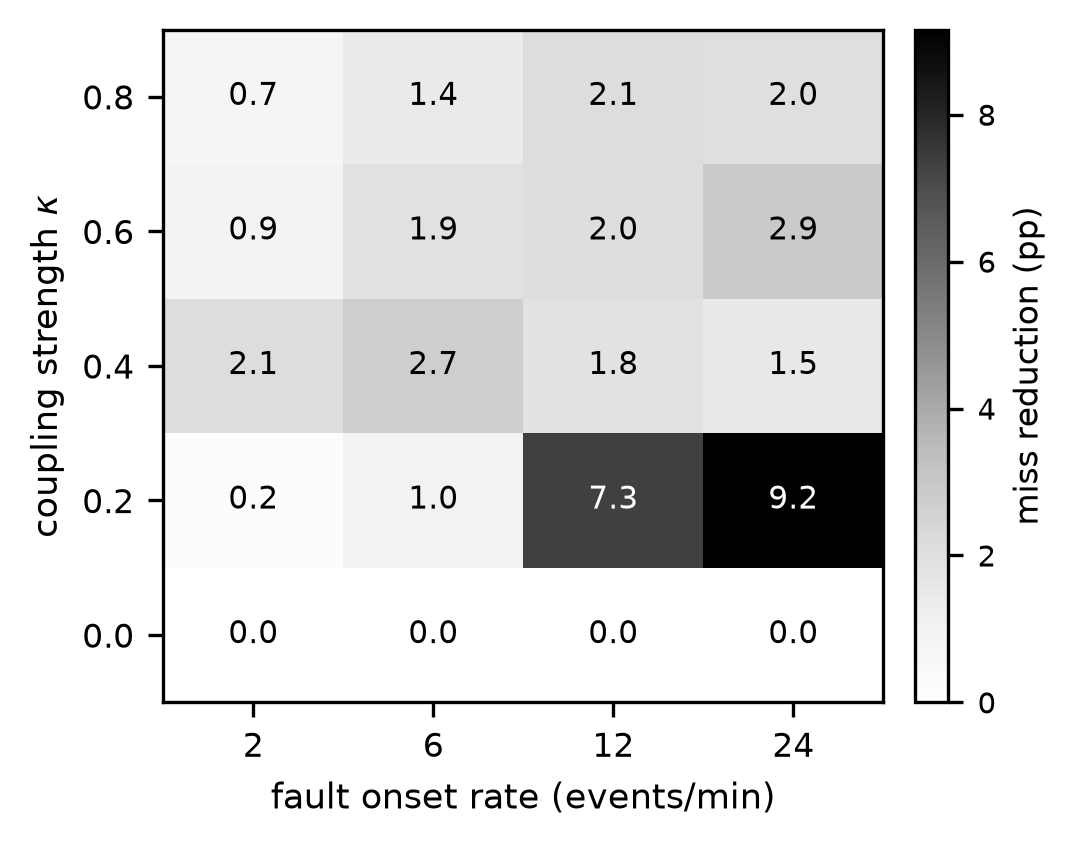
\includegraphics[width=\columnwidth]{fig_phase_diagram.png}
  \caption{RQ-H phase diagram (RADIATE fog): joint$-$decoupled
  deadline-miss reduction over a coupling$\times$onset-rate grid of
  controlled regimes. The $\kappa{=}0$ row is exactly zero (here and
  on all seven tracks); benefit grows only with coupling and onset
  rate -- the cleanest single statement of the mechanism.}
  \label{fig:phase}
\end{figure}

\subsection{RQ-A1/A2: Persistence and Dwell Time}

The HMM belief detector improves fault-detection balanced accuracy
(against independent onsets, not pseudo-GT) in every faulted track
($+3$ to $+8$ points, Table~\ref{tab:rqa1}) and reduces
config-switching significantly in three of five conditions (fog,
night, soiling), meeting the full pre-specified criterion (lower
switching at non-inferior accuracy) on night. It \emph{increases}
switching only on rain, where fast droplet flicker is
over-interpreted by HMM smoothing as sustained degradation -- a
fault-type-dependent result, not a flat negative, arguing for a
smoothing time-constant matched to the fault's temporal scale.

\begin{table}[htbp]
\caption{RQ-A1. Config-switching rate, belief vs.\ memoryless, and
detection balanced accuracy (independent onsets). $\Delta=$
memoryless$-$belief (positive = belief switches less); $^\ast$ CI
excludes zero.}
\label{tab:rqa1}
\centering
\footnotesize
\setlength{\tabcolsep}{3pt}
\begin{tabular}{lccccc}
\toprule
\textbf{Track} & \textbf{Belief} & \textbf{Mem.} &
\textbf{$\Delta$} & \textbf{bAcc$_{\text{bel}}$} & \textbf{bAcc$_{\text{mem}}$} \\
\midrule
D rain   & 0.020 & 0.010 & $-0.010^\ast$ & 0.884 & 0.854 \\
D snow   & 0.043 & 0.031 & $-0.012$      & 0.859 & 0.821 \\
D fog    & 0.037 & 0.047 & $+0.011^\ast$ & 0.752 & 0.668 \\
D night  & 0.050 & 0.074 & $+0.024^\ast$ & 0.825 & 0.794 \\
C soil   & 0.020 & 0.052 & $+0.031^\ast$ & 0.862 & 0.808 \\
\bottomrule
\end{tabular}
\end{table}

Under non-stationary fault arrival, model-derived hysteresis is
$\approx\!4\times$ more responsive than fixed hysteresis
(onset-to-reconfiguration lag $1.6$ vs.\ $6.6$ frames) but switches
$\approx\!30\%$ more; under stationary arrival the two are
indistinguishable, so the auto-tuned dwell matches hand-tuning
without manual calibration.

\subsection{RQ-Coupling: Does the Coupling Occur Naturally, and Does the Benefit Generalize?}
\label{sec:rqcoupling}

RQ-H is evaluated under an \emph{experimentally-imposed}
coupled/uncoupled schedule. We directly test whether that assumption
holds in un-manipulated data on RADIATE, adding \texttt{rain\_2\_0},
\texttt{rain\_3\_0}, \texttt{fog\_8\_0}, \texttt{fog\_8\_1} to the
four committed sequences (8 total). Table~\ref{tab:coupling}
summarizes five checks.

\textbf{(a) Measured coupling.} For every sequence we record real
per-frame latency and detection count (proxies independent of the
fault signals) and re-run RQ-H with contention scheduled from the
measured proxy instead of the fault label. Every correlation CI
centers near zero or the wrong sign and the de-circularized reduction
collapses to $\approx0.0$\,pp on all 8 sequences and both proxies:
the imposed regime \emph{constructs} the coupled scenario; we do not
find one already present in RADIATE by these proxies.

\textbf{(b) Cross-sequence consistency.} For rain and fog (3
independent sequences each) the per-sequence effect is positive in
all six traces and the cluster bootstrap stays entirely positive, but
the cross-sequence $t$-interval includes zero for both -- reported as
\emph{directionally consistent across tested sequences}, not as
generalizing.

\textbf{(c) Cross-sequence transfer of the full belief model.}
Fitting the \emph{entire} fault-belief estimator (the per-channel
switching HMMs) \emph{and} $\kappa$ on one sequence and testing on a
held-out one, the transferred detector still recovers faults
(balanced accuracy $0.65$--$0.90$ vs.\ $0.73$--$0.95$ native) and the
RQ-H reduction stays positive in all eight tested pairs and
significant in five -- including cross-\emph{condition} transfers
(rain$\rightarrow$fog $+7.8$\,pp, fog$\rightarrow$fog $+17.9$\,pp).
The whole belief model, not merely the scalar $\kappa$, generalizes
across trajectories, though the imposed-regime effect size can shrink
under transfer (e.g.\ fog $9.4\rightarrow4.4$\,pp).

\textbf{(d) A genuinely independent workload, multiple-testing
corrected.} Parts (a),(d) together run 24 tests (8 sequences
$\times$ 3 proxies: detections, latency, and a real, CPU-bound,
entirely separate ORB keypoint-matching workload independent of the
detector). We computed paired two-sided $p$-values directly from the
five seed-level differences of each test and applied
Benjamini--Hochberg across all 24 at $q{=}0.05$; the tests are not
fully independent (proxies share frames within a sequence, sequences
share a condition), a positive-dependence structure under which BH
still controls the false-discovery rate. A first run produced one
nominally positive result (\texttt{rain\_2\_0}, ORB proxy:
$+2.73$\,pp, $p{\approx}0.0024$), which narrowly missed its rank-1 BH
threshold ($0.05/24{\approx}0.0021$). Because the ORB proxy is timed
in real wall-clock and thus varies run to run, we then
\emph{re-measured} it: on replication the effect vanished entirely
($+0.00$\,pp, $p{=}1$; $P_c(\text{fault}){=}0.211 <
P_c(\text{nominal}){=}0.256$). After correction and replication,
\textbf{zero of 24 tests support naturally-occurring coupling}; the
one nominal positive was a measurement-timing artifact, exactly the
outcome multiple-testing discipline exists to catch.

\textbf{(e) Real annotations vs.\ pseudo-GT.} We projected RADIATE's
real radar-derived object annotations onto the camera image
(replicating the RADIATE SDK's radar-to-camera projection) and
computed real, class-agnostic detection F1 for all four configs on
RADIATE rain (500 frames). Real-GT F1 is far lower and flatter across
configs ($0.19$--$0.22$) than pseudo-GT F1 ($0.73$--$1.00$), the
config ranking does not match, and per-frame correlation between the
two is weak and sign-mixed. Coarser radar-projected boxes explain
part of the absolute gap, but the ranking mismatch means pseudo-GT is
an internal consistency check, not a validated accuracy proxy --
every accuracy and utility number inherits that limitation, while the
RQ-H deadline-miss numbers (Table~\ref{tab:rqh}) do not.

\begin{table}[htbp]
\caption{RQ-Coupling summary (RADIATE, 8 sequences). ``Result''
reports the honest, multiple-testing-aware outcome of each check.}
\label{tab:coupling}
\centering
\scriptsize
\setlength{\tabcolsep}{3pt}
\begin{tabular}{p{2.3cm}p{3.7cm}}
\toprule
\textbf{Check} & \textbf{Result} \\
\midrule
(a) Real coupling & Null: de-circ.\ $\Delta\approx0.0$\,pp vs.\ imposed $1.1$--$9.4$\,pp \\
(b) Cross-seq.\ consistency & Positive all 6 traces; $t$-CI incl.\ 0 at $n{=}3$ (not generalization) \\
(c) Full-model transfer & HMM+$\kappa$ trained on another sequence: sig.\ in 5/8 pairs, cross-condition too \\
(d) Independent workload (BH-corrected) & Null in 24/24 after correction; the one nominal positive failed replication \\
(e) Real-GT accuracy & Ranking mismatch; pseudo-GT is an internal check only \\
\bottomrule
\end{tabular}
\end{table}

Taken together: the joint policy produces nonnegative deadline-miss
reductions in all tested imposed-coupling conditions and the belief
model (HMM and $\kappa$) transfers across sequences, but after
correction and replication we
find \emph{no} confirmed case of naturally-occurring coupling in
un-manipulated RADIATE data. RQ-H is a proof of mechanism under a
controlled, experimentally-imposed regime -- not evidence that such
coupling, or the accuracy differences it is scored against, arise
naturally in the field.

% ---------------------------------------------------------------
\section{Discussion}
\label{sec:discussion}

The credibility of RQ-H rests on triangulation -- positive across
three datasets, two camera geometries, and multiple degradation
physics; exactly zero in every uncoupled control; harmless on the
fault-free trajectory -- isolating coupling as the driver rather than
an estimator or metric artifact. The benefit tracks fault
\emph{severity} (deadline-bindingness) more than frequency or
correlation, an interpretation inferred from condition-level outcomes
rather than a directly measured variable. Since the threshold rule
matches the noisy-OR, the supported claim is that \emph{using fault
belief to anticipate contention} helps -- not that the particular
noisy-OR belief-fusion algorithm is itself the advance.

\textbf{What the paper does and does not establish.} It establishes,
positively, (i) a real and portable mechanism -- where coupling exists,
a router that exploits it beats one that cannot by $1.1$--$9.4$\,pp, the
full belief model transfers across sequences and even weather
conditions, at negligible cost, with a falsification control at exactly
zero -- and (ii) a reusable, released evaluation pipeline
(imposed-schedule substrate, de-circularization, independent-workload
probe, multiple-testing protocol). What it does \emph{not} establish is
that the coupling premise holds in un-manipulated data: zero of 24
corrected tests show natural coupling, which we report plainly and equip
any deployment to test on its own traces before adopting the method.

\textbf{Limitations.} The evaluation is offline and trace-driven,
with a two-state, non-thermal contention model, evaluated only on an
Apple M5 -- not a shared embedded perception/planning/control stack.
Pseudo-GT is blind to systematic C1 error and only weakly validated
against real annotations (part e); every accuracy- or utility-based
conclusion should be read with that caveat, whereas the deadline-miss
conclusions (Table~\ref{tab:rqh}) do not depend on it. Moreover,
because pseudo-GT influences configuration ranking inside the
router's max-expected-accuracy objective, the deadline-miss result
establishes the timing mechanism but does not establish that the
selected configurations are optimal under real task accuracy.
The five seeds vary only injected measurement noise on identical real
frames, so seed CIs measure noise sensitivity, not cross-sequence
generalization -- which we separately bootstrap over 3 independent
trajectories per condition (directionally consistent across tested
sequences, not yet $t$-significant). RADIATE frames are rectified
left-camera only; WoodScape's temporal axis is dataset order, not
continuous video. Absolute latencies are dev-environment (Apple M5/MPS) driven by a
synthetic competitor, so the study does not yet exercise real silicon,
energy, or thermal contention as an HPEC evaluation ideally would. To
make that gap directly closable rather than aspirational, we release a
turnkey Jetson harness (\texttt{jetson\_harness.py}: real per-frame
latency, throughput, \texttt{tegrastats} energy per frame, a measured
co-running GPU competitor, and a sustained-load throttle check), so a
single real-silicon condition can be added without changing the
frontier or the routing code.

\textbf{Future work.} A factorial/cross-coupled HMM would upgrade
coupled-belief fusion to true joint belief-state estimation. Most
importantly: more independent sequences and repeated
\texttt{rain\_2\_0} trials to power the corrected real-coupling test;
real embedded contention on a Jetson to test for coupling on hardware
where it may plausibly arise; a full re-profiling of RQ-H on real
RADIATE annotations; and a closed-loop downstream-task evaluation
measuring task success rather than detector agreement.

% ---------------------------------------------------------------
\section{Conclusion}
\label{sec:conclusion}

We presented a belief-space perception router coupling sensor-fault
and compute-contention HMM beliefs via a noisy-OR term, reducing
deadline-miss rate by $1.1$--$9.4$\,pp when experimentally-imposed
coupling is enabled (significant in five of six conditions), while
every uncoupled control and the fault-free trajectory are exactly
zero -- a result that does not depend on pseudo-ground-truth
accuracy. Five further checks stress-test rather than assume the
coupling regime: after Benjamini--Hochberg correction and a
replication run, zero of 24 tests support naturally-occurring
coupling in 8 real sequences; the full belief model (HMM and
$\kappa$) nonetheless transfers across sequences, keeping the benefit
significant in five of eight held-out pairs including cross-condition
ones; and the pseudo-GT accuracy axis is an internal
consistency check only, so the timing mechanism is established but
config optimality under real task accuracy is not. The result is a portable, near-zero-cost coupling
mechanism with clean falsification controls and a reproducible
pipeline -- and one clearly scoped open question, whether the coupling
arises naturally, that the same pipeline lets any deployment answer on
its own traces.

% ---------------------------------------------------------------
\bibliographystyle{IEEEtran}
\bibliography{references}
\end{document}
